\documentclass{article}
\usepackage{graphicx}
\usepackage{booktabs}
\usepackage{array}
\usepackage{amsmath}
\usepackage{subcaption}
\usepackage{natbib}

\graphicspath{{figures/}}
\title{Group Effects of Idealized Debris Fields Driven by Tsunami-like Wave}
\date{September 2025}

\begin{document}

\maketitle

\section{Introduction}
Tsunami-driven debris fields pose significant hazards to coastal infrastructure, as they generate both short-duration impact loads and longer-lasting damming loads. Unlike hydrodynamic forces from waves alone, debris-induced forces are difficult to predict due to fluid - debris - structure - interactions. The complex interaction between fluid, structure, and debris creates significant uncertainty in estimating waterborne debris loads. Unlike single-object impacts, debris fields produce both sharp, short-duration impact forces and longer-lasting damming forces. Understanding how debris orientation, arrangement, and initial density influence these loading mechanisms is critical for resilient coastal infrastructure design. The objective of this study is to categorize group effects within debris fields and identify the governing mechanisms of debris–structure interaction. Large-scale flume experiments were conducted with systematically varied initial conditions, including debris orientation (longitudinal, transverse, and random), density, and size distribution (single vs.\ multi). Both unbroken and broken solitary waves were tested. The results highlight clear differences in impact amplification, damming behavior, and the role of randomness in debris loading.

Longitudinal debris alignments (i.e., oriented parallel to the incoming flow) tend to produce larger impacts than transverse configurations, while random fields display greater variability in impact magnitudes (Figures~\ref{fig:configurations} and \ref{fig:configurations_random}). Similarly, single-size debris groups behave differently than multi-size fields, particularly in their ability to form blockages and generate damming forces. Finally, surface area density---defined as the ratio of tightly packed debris cross-sectional area to the total spread area---controls the degree of clogging and thus the overall magnitude of structural loading.

\section{Literature Review} Post Tsunami surveys found that debris-driven damage has been a recurring failure mechanism. For example, reinforced concrete failures were observed during the 2004 Indian Ocean and 2011 Tohoku tsunamis, where large floating debris caused extensive structural damage \citep{Leonard2011,Akiyama2013,Suppasri2013}. Similarly, harbors along the U.S. west coast experienced tens of millions of dollars in damage attributed to floating debris \citep{Nakaso2011}. Recent reviews highlight the need for deeper study of how debris becomes mobilized and transfers momentum to structures, along with probabilistic approaches that reflect debris variability and source proximity, and more attention to the cumulative effects of repeated impacts and damming as debris clusters form \citep{nistorTsunamiDrivenDebrisMotion2017}.
Foundational studies approached debris impact from different perspectives. Haehnel and Daly \citep{Haehnel2004} performed flume experiments with flood-driven wooden debris and introduced single-degree-of-freedom (SDOF) formulations to reproduce collision behavior. In contrast, Naito et al. \citep{Naito2016} advanced a design-oriented framework that was incorporated into ASCE 7-16, where the Energy Grade Line (EGL) method was proposed to estimate debris velocities, impact forces, and critical impact elevations for coastal structures. Building on these efforts, Stolle et al. \citep{Stolle2018,Stolle2019} conducted flume experiments that demonstrated how impact and damming loads can be separated through signal decomposition and suggested an added mass term to better represent hydrodynamic effects. Recent research also highlights the importance of partially or fully submerged debris, which can significantly alter the magnitude and timing of structural loading. Extending this concept, Deschamps et al. \citep{deschampsNegativelyBuoyantDebris2025} investigated negatively buoyant debris under tsunami-like flows, showing that debris that sinks or stays near the bed can generate distinct impact and damming forces compared with floating debris, emphasizing the need to consider a full range of buoyancy conditions in structural load assessments.
Geometry and flow interaction have also been shown to matter, with scaled shipping container experiments demonstrating that debris impact velocity is reduced relative to the bore front due to stagnation and streamline effects near the structure \citep{Derschum2018}. Several studies have examined how debris is transported and accumulates in wave-driven flows, highlighting patterns of movement, clustering, and blockage formation. Laboratory investigations, such as Yao et al. \citep{Yao2014}, focused on the motion of model debris under solitary waves, providing insight into transport pathways and the stochastic nature of debris accumulation. Schmocker and Hager \citep{Schmocker2011} further demonstrated that accumulation occurs in two phases: an initial debris build-up that causes a major backwater rise, followed by formation of a debris carpet that extends downstream with only minor additional rise. Within the tested range, the primary factors controlling accumulation and backwater rise are the approach flow Froude number and debris volume, while debris type, mixture, and minor experimental factors have little effect. These studies provide valuable insight into debris behavior during inundation but generally do not quantify the resulting structural loads.

Building on these findings, more recent experimental work has directly addressed multi-debris impacts and damming on structures. Shekhar et al. \citep{Shekhar2020} used scaled, neutrally buoyant blocks to study how debris clusters interact with a vertical test structure under tsunami-like flows, capturing both the initial impact and subsequent low-frequency damming forces. Large-scale flume experiments at Oregon State University (OSU) extended this work by measuring impact and damming forces under varying debris densities, orientations, and flow conditions, while also evaluating the applicability of ASCE 7-22 tsunami load provisions \citep{Doyle2024}. Complementary studies have used flume experiments to improve numerical models of debris-field interactions and their effects on structures \citep{Bonus2022, bonusTsunamiDebrisMotion2025}. Bonus et al. (2025) compared simulations with scaled flume tests, helping to refine predictions of debris movement, stacking, and impacts in a simplified port setting.

\begin{figure}[htbp]
    \centering
    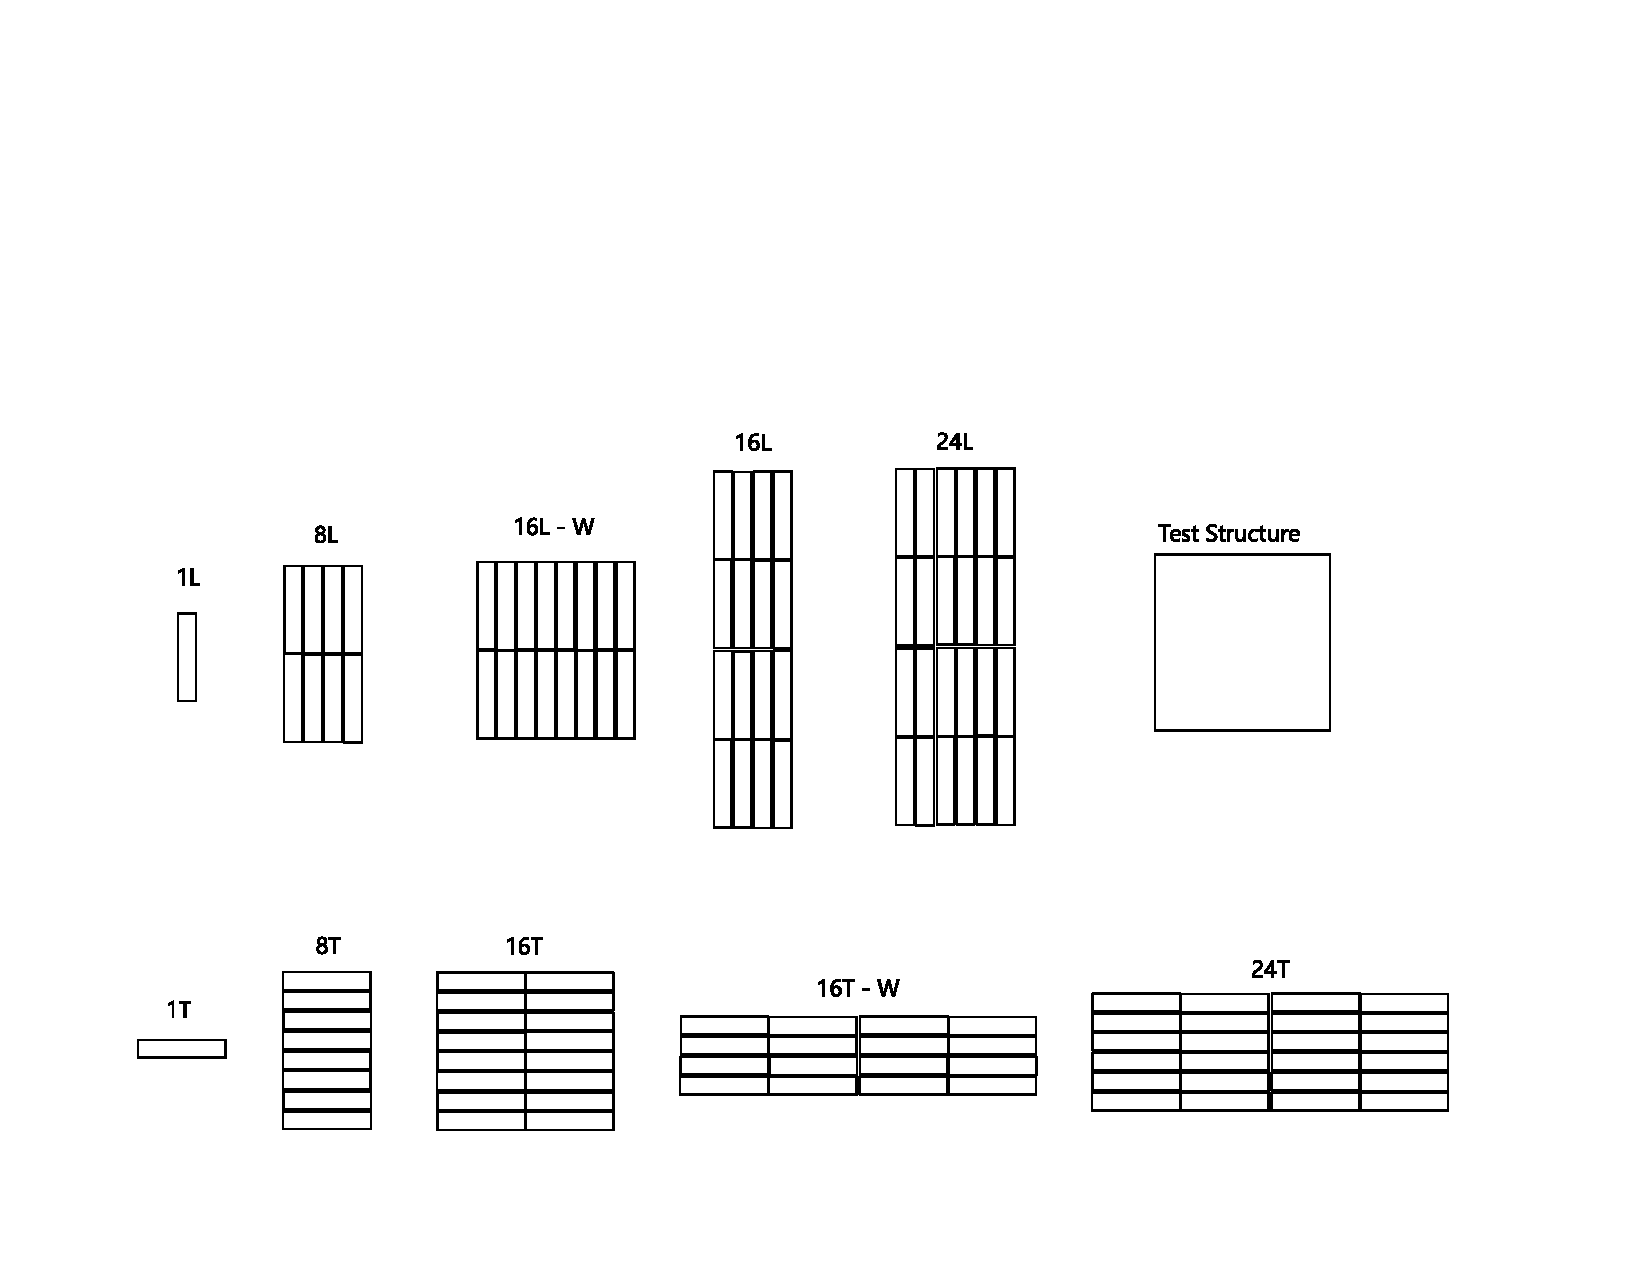
\includegraphics[width=0.8\textwidth]{Configurations.jpg}
    \caption{Regular configurations.}
    \label{fig:configurations}
\end{figure}

\begin{figure}[htbp]
    \centering
    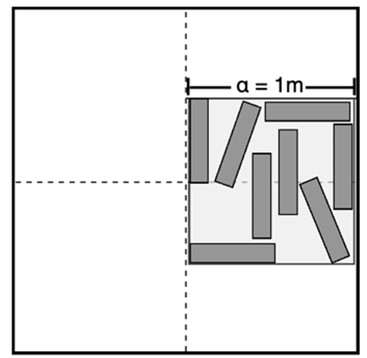
\includegraphics[width=0.48\textwidth]{configurations_rand.jpg}
    \caption{Random configurations.}
    \label{fig:configurations_random}
\end{figure}

\begin{figure}[htbp] \centering 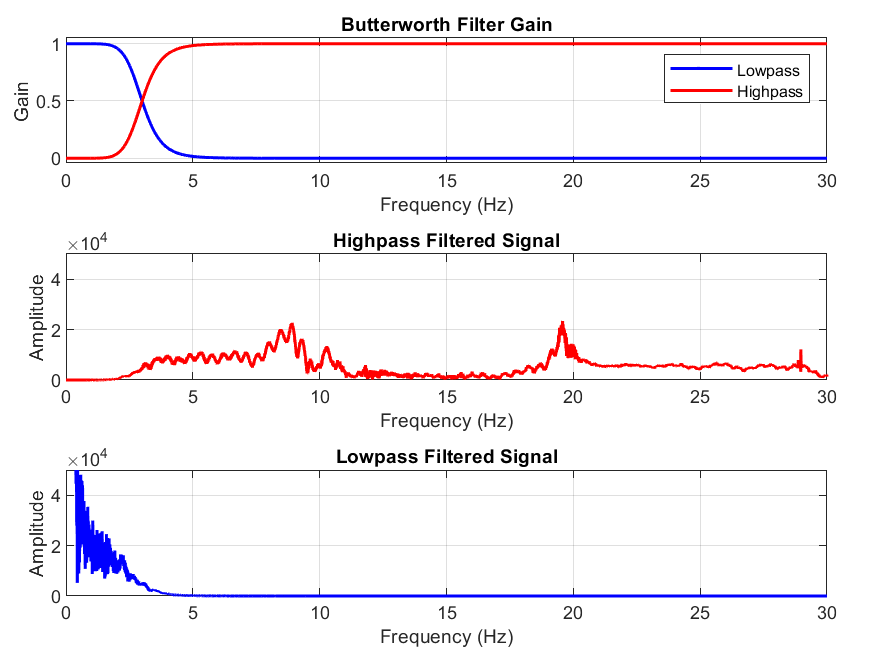
\includegraphics[width=0.8\textwidth]{high_low_pass.png} \caption{Force decomposition using Butterworth filters.} \label{fig:high_low_pass} \end{figure}

\section{Testing Methodology}
The experiments were conducted in a large-scale tsunami flume equipped with a rigid structure placed at mid-flume. Two types of solitary waves were investigated: unbroken solitary waves and broken solitary waves. The present study focuses exclusively on the unbroken solitary wave cases, which provide a clearer baseline for analyzing debris-induced loading mechanisms. Debris fields were prepared in three general configurations: regular longitudinal layouts, regular transverse layouts, and random arrangements that included both single-size and multi-size distributions.

To analyze force signals, the time histories were decomposed using Butterworth filters. High-pass filtering was applied to isolate short-duration impact peaks, while low-pass filtering was used to extract long-duration damming forces (Figure~\ref{fig:high_low_pass}). This filtering approach allowed us to distinguish between transient impact loads and sustained blockage-induced forces, ensuring that each mechanism could be evaluated independently.

Representative examples of impact and damming time histories are shown for both small debris fields (1L) and large debris fields (24L) in Figures~\ref{fig:timehist_combined} and \ref{fig:timehist_damming_combined}. The differences in the magnitude and duration of forces across these cases illustrate how debris quantity strongly alters the loading signature.

\begin{figure}[h!]
    \centering
    \begin{subfigure}[b]{0.48\textwidth}
        \centering
        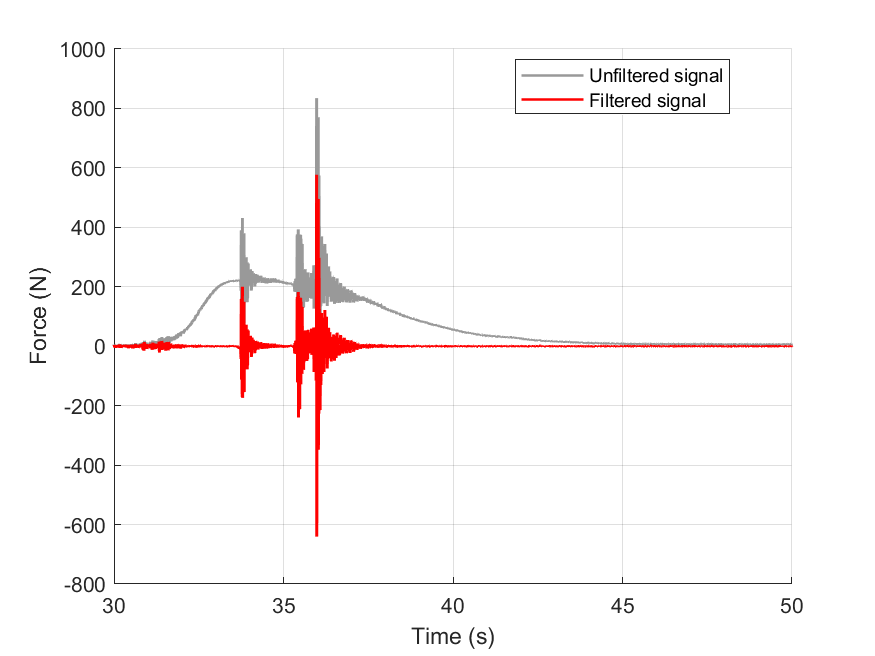
\includegraphics[width=\textwidth]{Reg_Lift_U_1_L_D__Masters_NHERIDeprisImpact2_goodtests_Reg_Lift_U_1_L_Trial04_Peak.png}
        \caption{1L debris.}
        \label{fig:timehist_1L_peak}
    \end{subfigure}
    \hfill
    \begin{subfigure}[b]{0.48\textwidth}
        \centering
        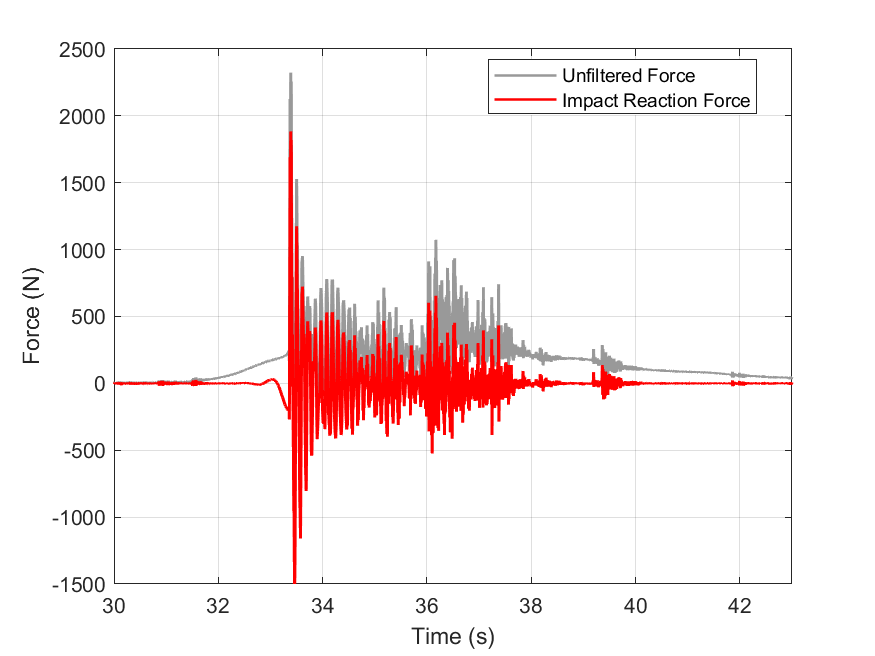
\includegraphics[width=\textwidth]{Reg_Lift_U_24_L_D__Masters_NHERIDeprisImpact2_goodtests_Reg_Lift_U_24_L_Trial04_Peak.png}
        \caption{24L debris.}
        \label{fig:timehist_24L_peak}
    \end{subfigure}
    \caption{Force time histories.}
    \label{fig:timehist_combined}
\end{figure}

\begin{figure}[h!]
    \centering
    \begin{subfigure}[b]{0.48\textwidth}
        \centering
        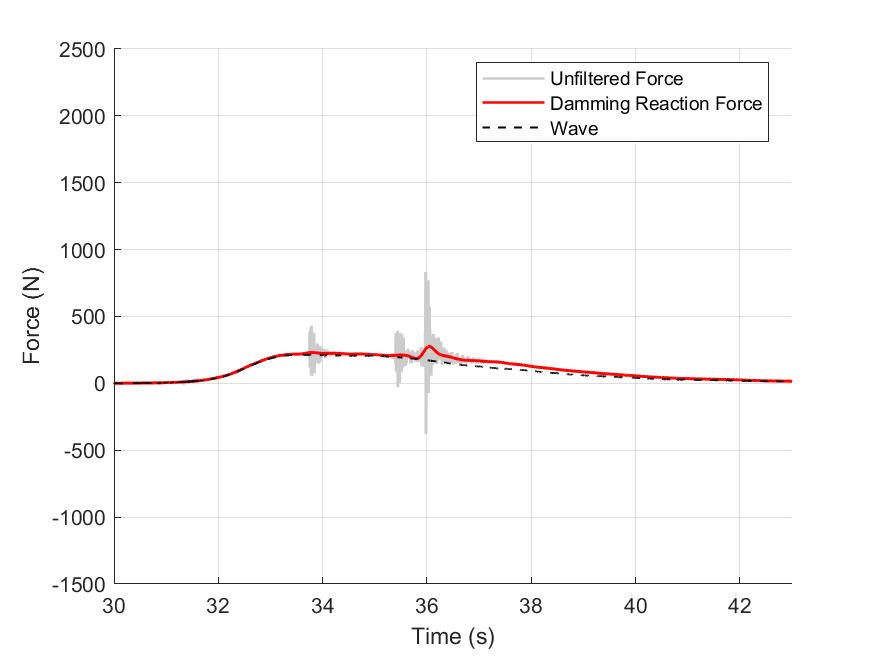
\includegraphics[width=\textwidth]{Reg_Lift_U_1_L_D__Masters_NHERIDeprisImpact2_goodtests_Reg_Lift_U_1_L_Trial04_Damming.png}
        \caption{1L debris.}
        \label{fig:timehist_1L_damming}
    \end{subfigure}
    \hfill
    \begin{subfigure}[b]{0.48\textwidth}
        \centering
        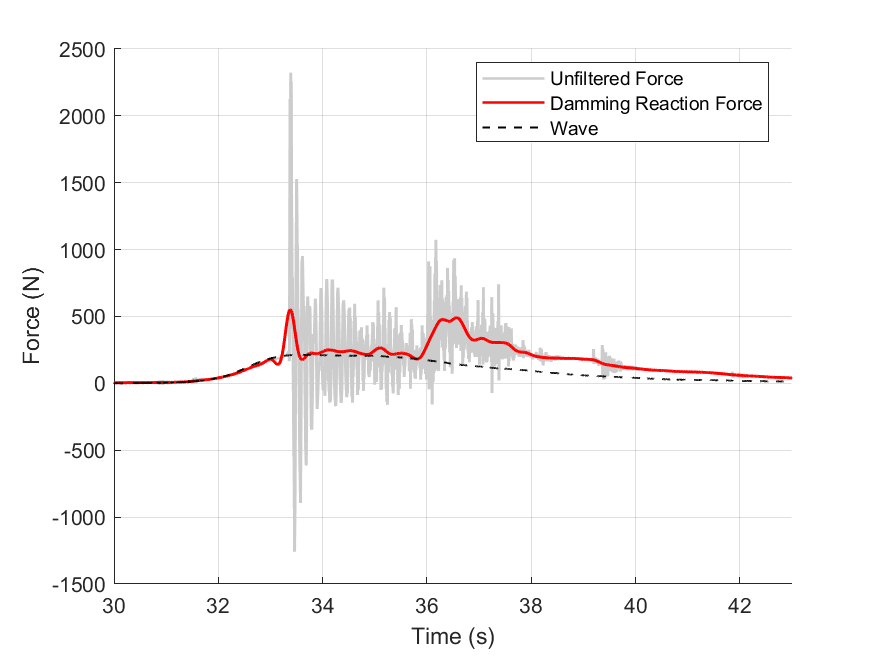
\includegraphics[width=\textwidth]{Reg_Lift_U_24_L_D__Masters_NHERIDeprisImpact2_goodtests_Reg_Lift_U_24_L_Trial04_Damming.png}
        \caption{24L debris.}
        \label{fig:timehist_24L_damming}
    \end{subfigure}
    \caption{Damming force time histories.}
    \label{fig:timehist_damming_combined}
\end{figure}

\section{Impact and Damming Reaction Forces}
Video evidence combined with filtered force records revealed that debris impacts occur in two distinct stages. The first stage is the initial unsubmerged impact, where debris pieces strike the structure immediately upon arrival (Figure~\ref{fig:first_impact}). These impacts are characterized by a sharp and simultaneous peak, particularly in longitudinal configurations. The second stage consists of later submerged impacts, which arise when debris recirculates downstream and strikes the structure again under partially submerged conditions (Figure~\ref{fig:second_impact}). Unlike the first impact, these later impacts are more scattered, chaotic, and prolonged, especially in tests involving larger numbers of debris pieces. The distinction between first and later impacts proved consistent across all debris types and configurations, underscoring the need to treat these two stages as separate mechanisms in structural analysis.

\begin{figure}[htbp]
    \centering
    \begin{subfigure}[b]{0.48\textwidth}
        \centering
        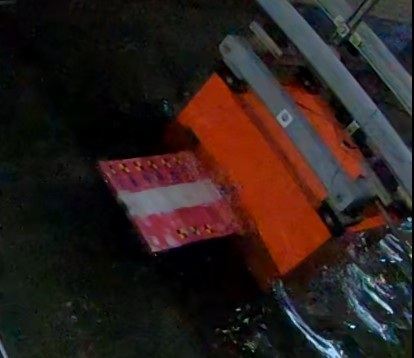
\includegraphics[width=\textwidth]{first_impact.jpg}
        \caption{First unsubmerged impact.}
        \label{fig:first_impact}
    \end{subfigure}
    \hfill
    
    \begin{subfigure}[b]{0.48\textwidth}
        \centering
        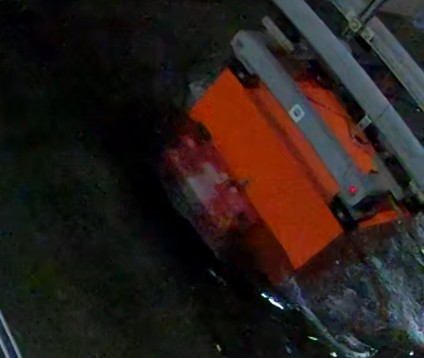
\includegraphics[width=\textwidth]{second_impact.jpg}
        \caption{Later submerged impact.}
        \label{fig:second_impact}
    \end{subfigure}
    \caption{Impact events: (a) initial unsubmerged impact and (b) later submerged impact.}
    \label{fig:impact_combined}
    
\end{figure}
\section{Results: Regular Configurations}

\subsection{Impact Forces} In regular configurations, the first impact peaks scaled approximately linearly with the number of debris pieces (Figure~\ref{fig:firstpeak_regular_split}). This relationship was clear across both longitudinal and transverse layouts, although the absolute magnitudes differed. Later impacts, by contrast, exhibited nonlinear behavior, showing growth that eventually saturated as debris counts increased (Figure~\ref{fig:laterpeak_regular_split}). This saturation suggests that once a certain number of pieces are present, additional debris no longer contributes significantly to impact loading because not all debris can strike the structure simultaneously.

Longitudinal arrangements consistently produced the highest impact forces. This trend is attributed to direct alignment with the incoming wave, which promoted synchronous collisions. In contrast, transverse layouts yielded smaller impact peaks. The orientation caused debris to spread laterally, allowing the intervening water layer to cushion impacts and thereby reducing peak magnitudes.

For specific cases such as the 24T and 16T2 tests, the lateral extent of the debris field exceeded the structure’s width. Consequently, not all debris pieces were able to make contact with the structure. To address this limitation, the data were adjusted to reflect the effective contact area (Figures~\ref{fig:firstpeak_regular_split} and \ref{fig:laterpeak_regular_split}). This adjustment allowed direct comparison between different configurations. Interestingly, when adjusted, the 24T case behaved similarly to a 12T case in terms of effective contact, although the hydrodynamic influence of the larger debris count still altered the flow field. This explains why the adjusted forces in large debris fields sometimes appeared lower than in smaller cases.

The overall trends are illustrated in Figure~\ref{fig:firstpeak_medians_trend}, which shows that normalized first impact forces exhibit a clear linear trend with increasing debris number. This behavior confirms that debris quantity is a first-order driver of peak impact forces in regular configurations.
\begin{figure}[htbp]
    \centering
    \begin{subfigure}[t]{0.48\textwidth}
        \centering
        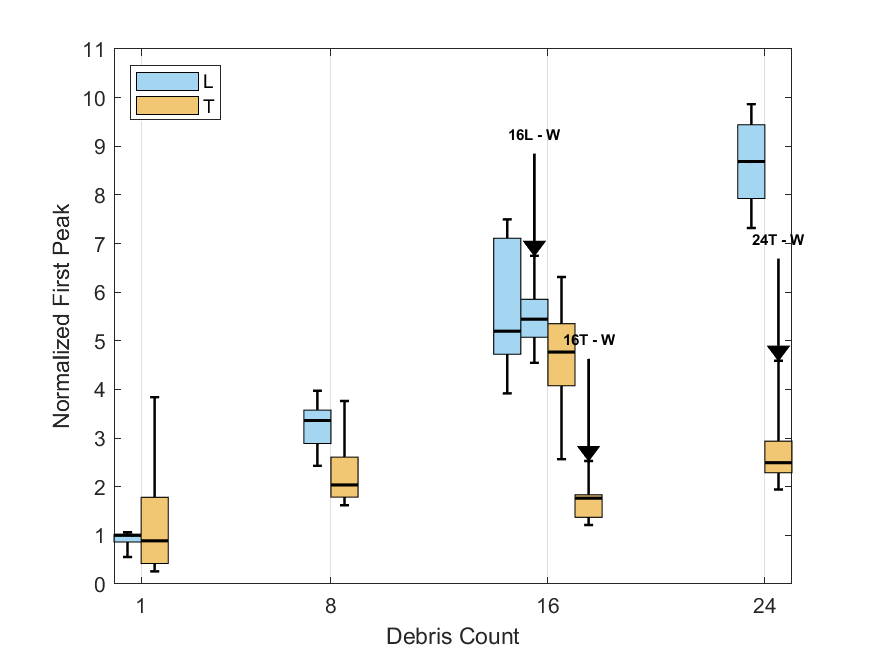
\includegraphics[width=\textwidth]{FirstPeak_Regular_SplitByTrial.png}
        \caption{Original.}
        \label{fig:firstpeak_regular_original}
    \end{subfigure}
    \hfill
    \begin{subfigure}[t]{0.48\textwidth}
        \centering
        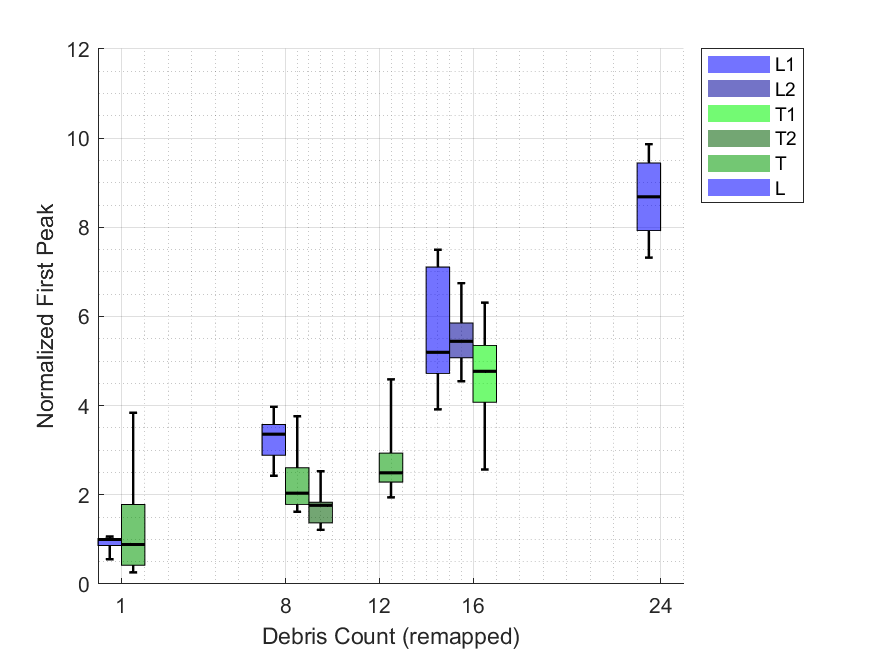
\includegraphics[width=\textwidth]{FirstPeak_Regular_RemappedT.png}
        \caption{adjusted.}
        \label{fig:firstpeak_regular_remap}
    \end{subfigure}
    \caption{First peak forces in regular configurations split by orientation and width.}
    \label{fig:firstpeak_regular_split}
\end{figure}

\begin{figure}[htbp]
    \centering
    \begin{subfigure}[t]{0.48\textwidth}
        \centering
        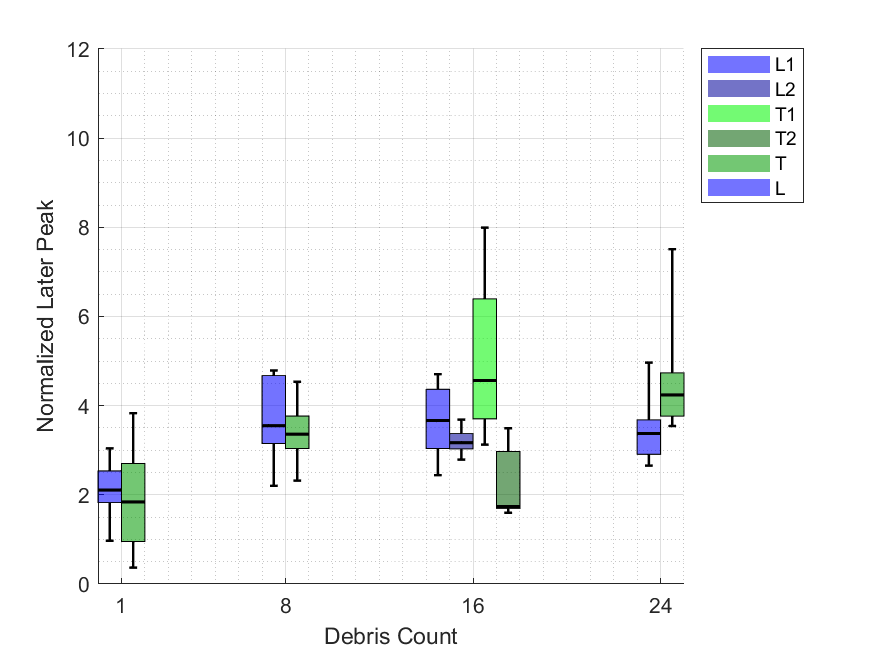
\includegraphics[width=\textwidth]{LaterPeak_Regular_SplitByTrial.png}
        \caption{Original.}
        \label{fig:laterpeak_regular_original}
    \end{subfigure}
    \hfill
    \begin{subfigure}[t]{0.48\textwidth}
        \centering
        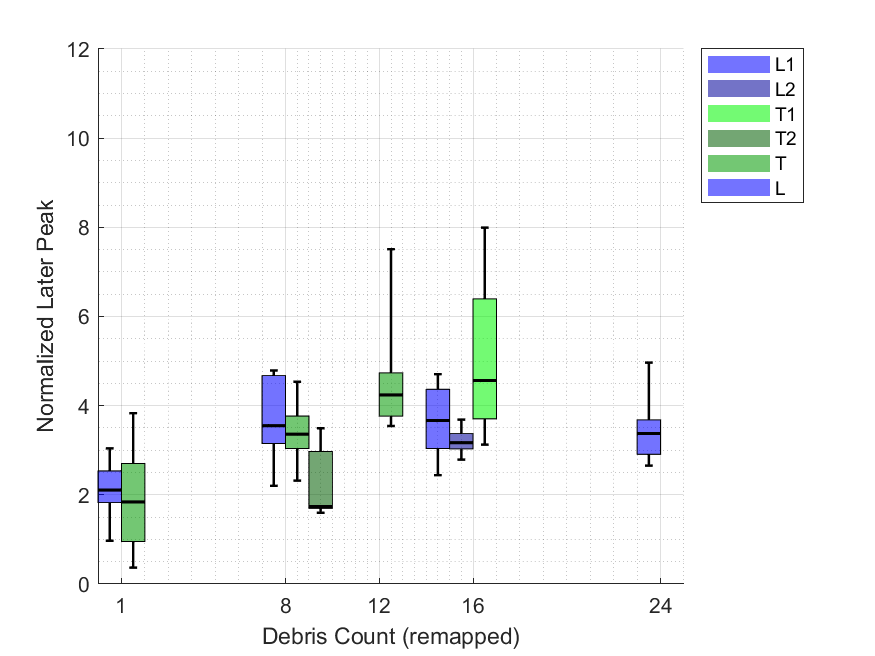
\includegraphics[width=\textwidth]{LaterPeak_Regular_RemappedT.png}
        \caption{adjusted.}
        \label{fig:laterpeak_regular_remap}
    \end{subfigure}
    \caption{Later peak forces in regular configurations: (a) original trials, (b) adjusted trials.}
    \label{fig:laterpeak_regular_split}
\end{figure}

\subsection{Damming Forces} Damming forces were extracted from low-pass filtered signals, capturing the sustained blockage loads. In single-size debris fields, increasing surface area density promoted tighter packing of debris, which facilitated stable jamming and produced higher damming forces (Figures~\ref{fig:damming_regular_split}). Comparisons between longitudinal and transverse orientations revealed that while overall magnitudes were broadly similar, transverse configurations produced higher damming loads once debris counts exceeded eight. This trend indicates that longitudinal configurations dominate impact peaks, while transverse configurations dominate damming forces. Nonlinear saturation was also observed: as debris counts increased, damming loads eventually plateaued. This behavior parallels the nonlinear growth of later impact peaks and is attributed to both complete blockage conditions and recirculating debris that no longer contributed significantly to additional damming loads.
\begin{figure}[htbp]
    \centering
    \begin{subfigure}[t]{0.48\textwidth}
        \centering
        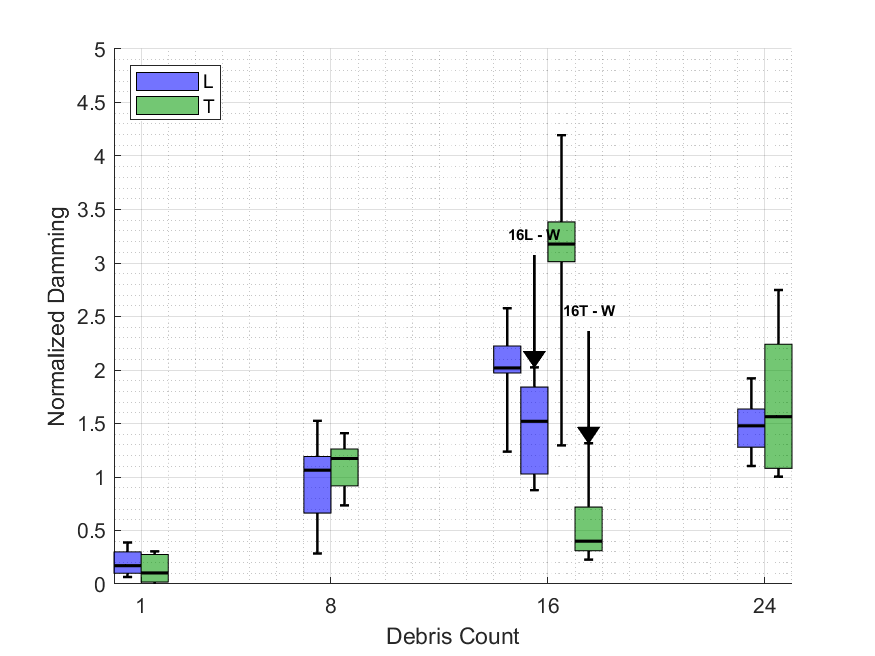
\includegraphics[width=\textwidth]{Damming_Regular_SplitByTrial.png}
        \caption{Original.}
        \label{fig:damming_regular_original}
    \end{subfigure}
    \hfill
    \begin{subfigure}[t]{0.48\textwidth}
        \centering
        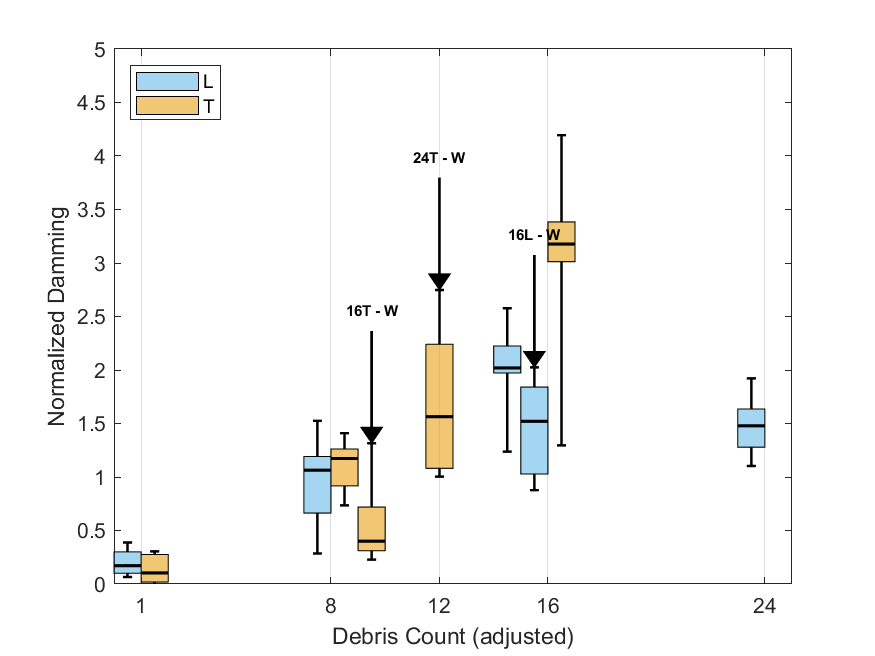
\includegraphics[width=\textwidth]{Damming_Regular_L_T_SplitByTrial_Remapped.png}
        \caption{adjusted.}
        \label{fig:damming_regular_remap}
    \end{subfigure}
    \caption{Damming forces in regular configurations: (a) original trials, (b) adjusted trials.}
    \label{fig:damming_regular_split}
\end{figure}

\section{Results: Random Configurations}
Random debris fields, in which debris pieces are distributed without a regular orientation, are first analyzed in terms of unaltered impact and damming forces as a function of the total number of debris pieces and the surface area density within the debris frame. Debris is initially arranged within a rectangular frame, and higher surface area densities require pieces to be more closely packed, which often causes the frame to span a wider section of the flume when lifted. Subsequent adjustments account for partial debris contact using video-derived impact probabilities, and the analysis concludes with corrected median values that isolate the contributions of only the largest debris blocks in multi-size fields, providing insight into the limited effect of smaller pieces on structural loading.

\subsection{Impact Forces} 
Random debris configurations produced more scattered data compared to regular arrangements. The peak magnitudes were generally smaller, but variability increased considerably. Multi-size debris fields consistently generated lower impact magnitudes than single-size fields because the smaller blocks contributed less momentum. This effect was particularly pronounced in tests with larger debris counts, where multiple smaller blocks often struck separately rather than in a single coherent cluster.

The unaltered gradient plots show these differences most clearly. In the first impact peaks, single-sized debris fields consistently yielded higher forces than multi-sized fields, and increasing surface area density raised the magnitude of impact (Figure~\ref{fig:random_peaks_first}). Later impact peaks, occurring after initial contact and partial submergence, showed only a slight increase with debris count (Figure~\ref{fig:random_peaks_later}). In these later impacts, density effects were visible for single-sized debris fields but largely absent in multi-sized cases.

\begin{figure}[htbp]
    \centering
    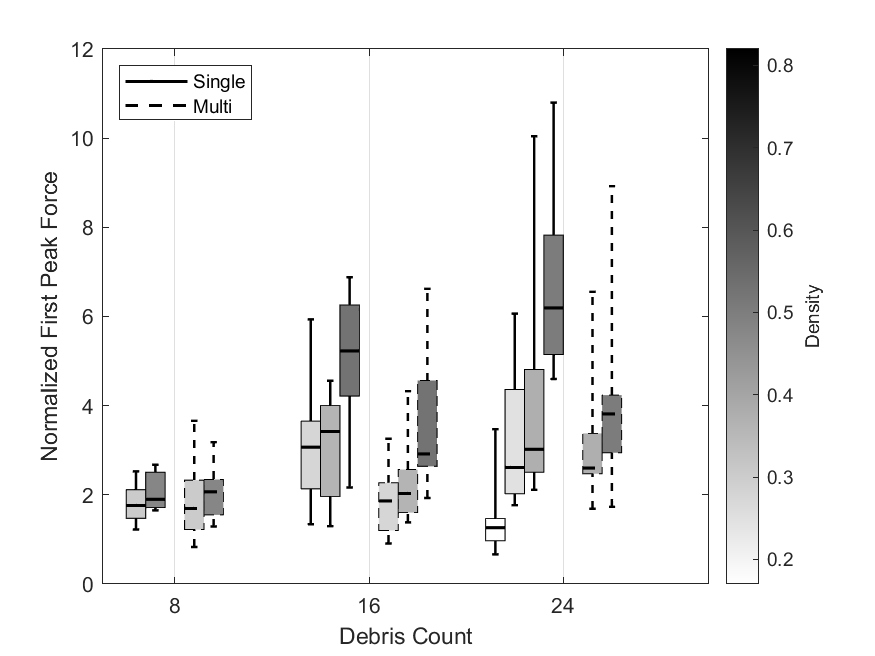
\includegraphics[width=0.8\textwidth]{First_Peak_Random_Single_vs_Multi_ByDensityGradient.png}
    \caption{First impact forces in random fields. Single-sized debris fields consistently yield higher impact forces than multi-sized debris fields. Surface area density furthermore affects impact magnitude, with lower densities resulting in smaller peak forces.}
    \label{fig:random_peaks_first}
\end{figure}

\begin{figure}[htbp]
    \centering
    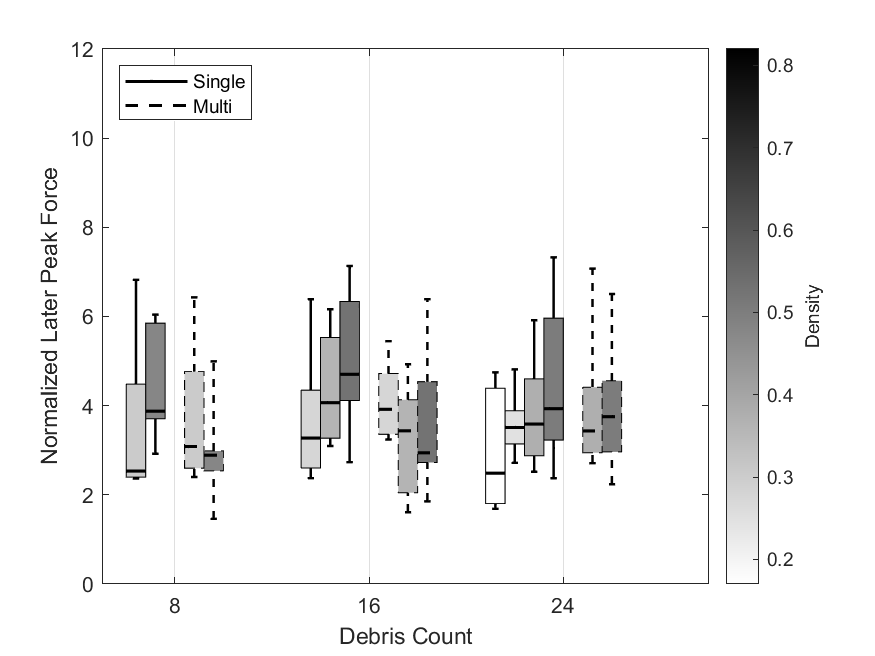
\includegraphics[width=0.8\textwidth]{Later_Peak_Random_Single_vs_Multi_ByDensityGradient.png}
    \caption{Later impact forces in random debris fields show only a slight increase in reaction force with increasing debris count. The effect of density is present in single-sized debris fields, while in multi-sized fields density shows no effect.}
    \label{fig:random_peaks_later}
\end{figure}

A critical adjustment became necessary because the pre-release debris frame often exceeded the structure’s width when spanning higher densities or debris counts. This geometry meant that not all pieces could reach the structure, and some pieces were effectively excluded from impact. Video analysis confirmed this by counting the actual number of blocks making contact with the structure. From these counts, an \emph{impact probability} was derived, which decreased proportionally as the frame widened relative to the structure (Figure~\ref{fig:impact_probabilities}). To account for this effect, a linear correction was applied to all trials: the effective number of impacting pieces was defined as the nominal debris count multiplied by the ratio of structure width to frame width. This correction ensured comparability between different configurations and removed artificial reductions in observed force magnitudes.

\begin{figure}[htbp]
    \centering
    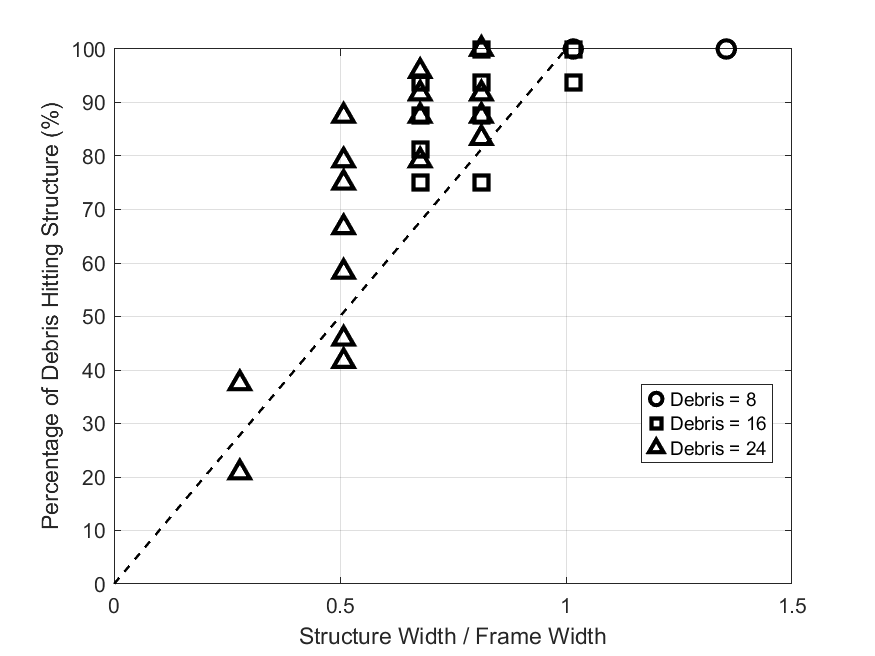
\includegraphics[width=0.8\textwidth]{Impact_probabilities.png}
    \caption{Impact probabilities across random trials. Increasing the frame width relative to the structure width proportionally decreases the percentage of debris impacting the structure.}
    \label{fig:impact_probabilities}
\end{figure}

The corrected median plots reflect these adjustments. Figure~\ref{fig:random_first_median_adjusted} shows normalized first impact peaks after applying the width-based correction. Single-sized debris fields again produce higher forces than multi-sized fields, with forces rising until saturation as debris counts increase. For multi-sized fields, additional filtering was carried out to isolate only the large blocks. This revealed that the largest blocks generated slightly higher impact peaks than the single-sized debris, while the smaller blocks added only a modest contribution. Thus, while small pieces do matter, the dominant contribution to peak loading comes from the larger blocks.

The same trends were observed in the later impact peaks (Figure~\ref{fig:random_later_median_adjusted}). Single-sized debris produced consistently stronger forces, while multi-sized debris showed weaker responses. Filtering for large blocks confirmed that smaller debris added only marginally to the total force.

\begin{figure}[htbp]
    \centering
    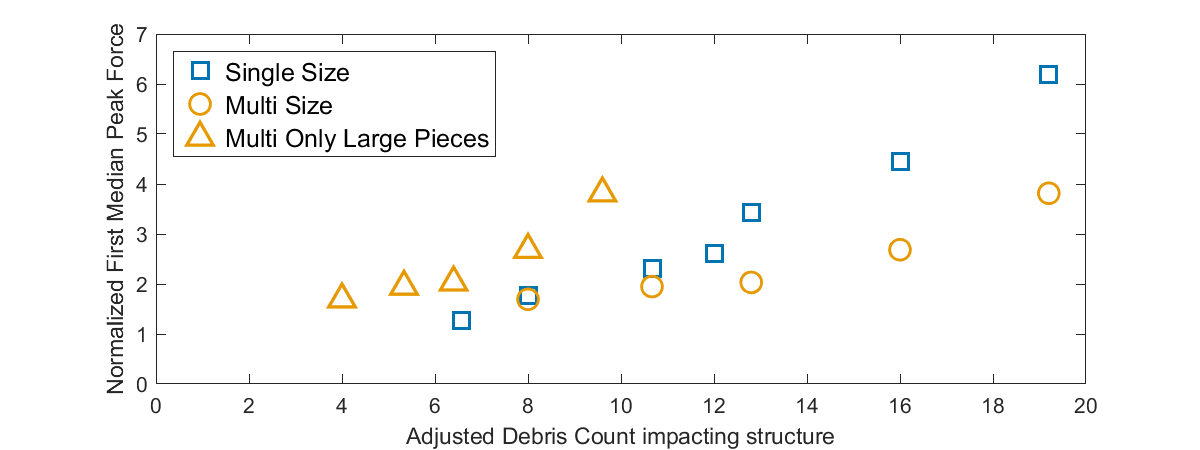
\includegraphics[width=0.75\textwidth]{First_Peak_Median_Single_vs_Multi_Adjusted.png}
    \caption{Median normalized first impact peaks in random fields after adjustment by structure width. Single-sized debris fields generate higher impact peaks than multi-sized fields. Filtering only the large blocks in multi-size fields reveals that smaller blocks provide additional impact contribution, but only modestly.}
    \label{fig:random_first_median_adjusted}
\end{figure}

\begin{figure}[htbp]
    \centering
    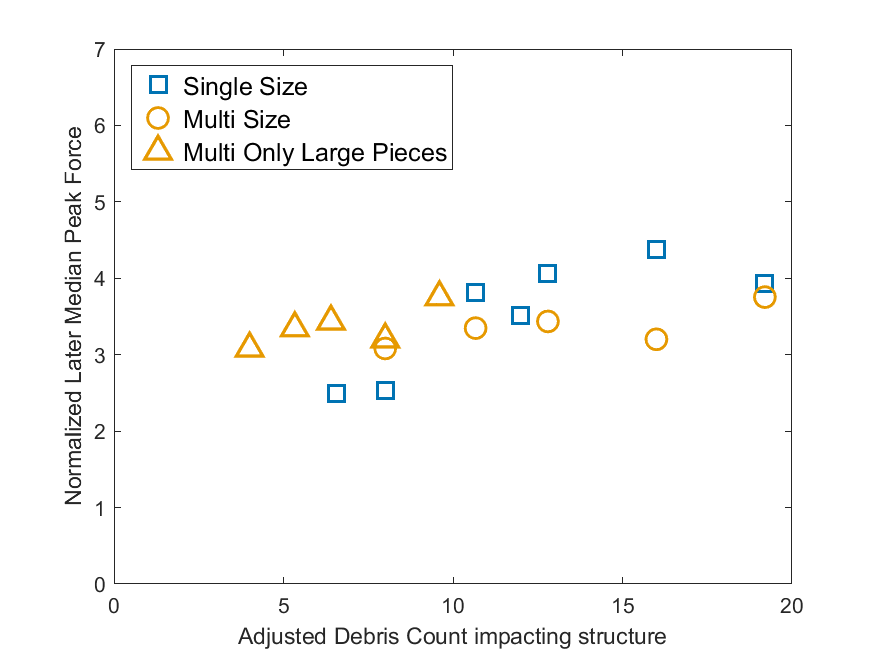
\includegraphics[width=0.75\textwidth]{Later_Peak_Median_Single_vs_Multi_Adjusted.png}
    \caption{Median normalized later impact peaks in random fields after adjustment by structure width. Single-sized debris fields produce higher peaks than multi-sized fields, while filtering for large blocks in multi-size fields again shows that the smaller blocks contribute only marginally to total forces.}
    \label{fig:random_later_median_adjusted}
\end{figure}

\subsection{Damming Forces} 
In random configurations, damming forces followed a different pattern compared to regular layouts. The unaltered gradient plot (Figure~\ref{fig:random_damming_gradient}) shows that single-sized debris fields generated higher sustained loads than multi-sized fields, with surface area density promoting stronger clustering and jamming. In contrast, multi-sized fields disrupted jamming, allowing bypass flow and weakening density effects.

\begin{figure}[htbp]
    \centering
    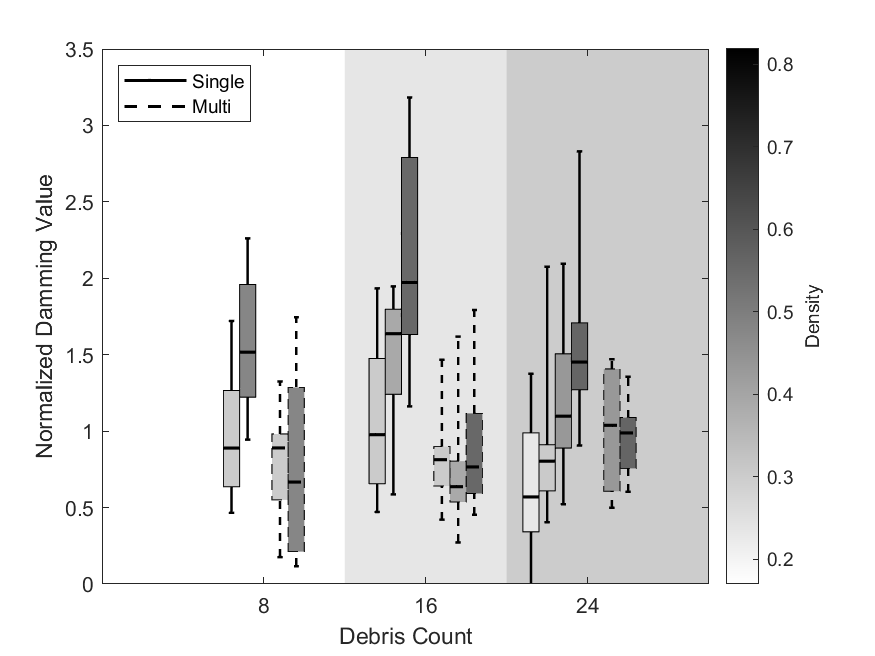
\includegraphics[width=0.8\textwidth]{Damming_Random_Single_vs_Multi_ByDensityGradient.png}
    \caption{Normalized damming forces in random debris fields. Single-sized debris fields consistently yield higher damming forces than multi-sized debris fields. Surface area density further increases sustained loads in single-size cases but has little to no effect in multi-size fields.}
    \label{fig:random_damming_gradient}
\end{figure}

The corrected median values (Figure~\ref{fig:random_damming_median_adjusted}) show a noteworthy consistency: across all densities and debris counts, normalized damming forces remained close to a 100\% increase over baseline wave loading. This indicates that while density and debris size distribution influenced variability, the sustained force contribution of damming in random fields remained broadly similar across conditions. In other words, random configurations consistently doubled the baseline wave load, with single-size fields amplifying clustering effects and multi-size fields reducing them through blockage disruption.

\begin{figure}[htbp]
    \centering
    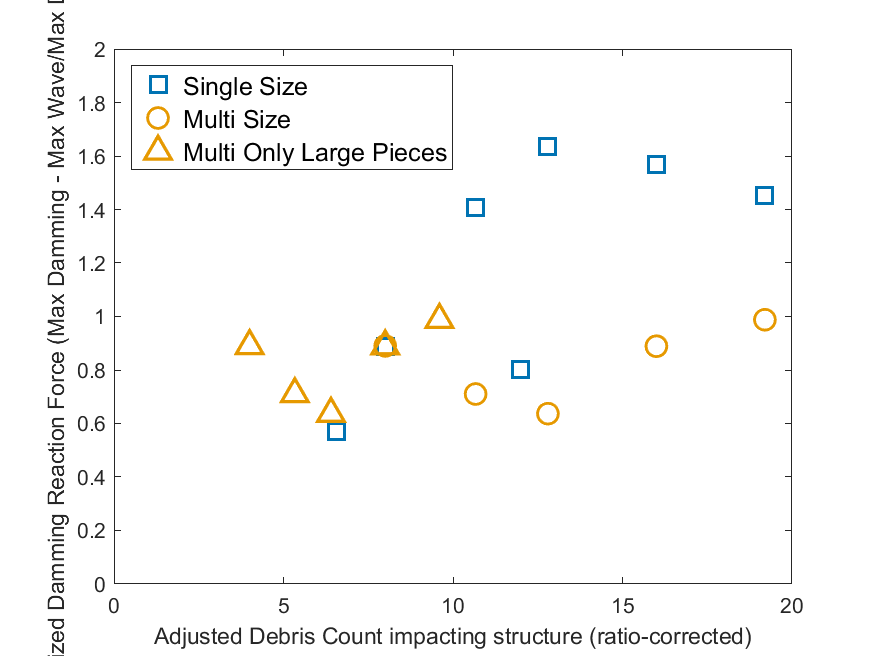
\includegraphics[width=0.75\textwidth]{Damming_Median_Single_vs_Multi_Adjusted.png}
    \caption{Median normalized damming forces in random fields, adjusted by structure width. Across all conditions, damming forces remain around a 100\% increase over wave-only loading, with stronger density effects in single-size fields and weaker effects in multi-size fields due to disrupted jamming.}
    \label{fig:random_damming_median_adjusted}
\end{figure}


\section{Conclusions} The experiments demonstrate that debris orientation, size distribution, and density are all critical factors in determining the forces exerted on coastal structures. Longitudinal groups generated the largest impact peaks, while transverse groups dominated sustained damming forces. Random and multi-size fields generally produced smaller and more variable loads, highlighting their reduced capacity for synchronous impacts and stable blockages. Surface area density strong

\section{Limitations}
Several limitations of this study should be acknowledged. First, because of the high impact forces generated during the tests, it was not possible to directly record loads at the front of the flume. As a result, the measurements represent reaction forces transmitted through the structure, which inevitably include contributions from structural vibrations and cannot fully isolate the instantaneous impact loads. Second, the geometry of the flume influenced the flow conditions. In particular, confinement effects from the side walls amplified cushioning by the water layer, altering the magnitude and duration of impacts compared to conditions in an open channel or coastal environment. Third, the relative widths of the debris fields and the test structure constrained the representativeness of certain configurations. When the debris field exceeded the structure width, only partial contact was achieved, requiring data remapping to allow meaningful comparison across trials. Finally, the practical limits on the number of debris pieces that could be deployed restricted the parameter space explored in the experiments. While the tested cases captured a range of densities, sizes, and orientations, the upper bound of debris group sizes was necessarily limited, leaving open the possibility that larger-scale accumulations could produce different scaling relationships. Addressing these constraints in future studies will be critical to improving the generalization of the results and to refining debris-impact models for coastal infrastructure design.

\section{References}
\bibliographystyle{plainnat}  
\bibliography{Thesis}

\end{document}
